\documentclass[en,license=none]{../../../eplnotes}

\usepackage{ragged2e}

\newcolumntype{L}[1]{>{\justify\let\newline\\\arraybackslash\hspace{0pt}}m{#1}}
\newcolumntype{C}[1]{>{\centering\let\newline\\\arraybackslash\hspace{0pt}}m{#1}}
\newcolumntype{R}[1]{>{\justify\let\newline\\\arraybackslash\hspace{0pt}}m{#1}}

\hypertitle{Computer networks: configuration and management}{7}{INGI}{2142}
{Houtain Nicolas, Gorby Nicolase Kabasele Ndondas, Luis Tascon Gutierrez}
{Olivier Bonaventure}

%TODO put in order the following sections:
% 1 BGP
% 2 MPLS
% 3 MPLS-VPN
% 4 Failures
% 5 Traffic control
% 6 Multicast
% 7 Segment Routing
% (8 abbreviations)

\section{Evolution of the internet QoS and support for soft real-time
	applications}

\textit{In this paper, we review several mechanisms and frameworks proposed to provide network and application-level quality of service (QoS) in the next-generation Internet.}


\subsection{Internet QoS}

Real-time applications require special support from network such
as reliability, timeliness and guaranteed delivery. The degree of
tolerance to each of these parameters varies from one application to
another.

Most of application are based on the TCP which provides reliable data
delivery service \textbf{without guaranteeing any delay and bounds}.


\begin{description}
	\item[QoS] : the capability to provide resource
	assurance and service differentiation in a network.
\end{description}

\subsubsection{Real-time application and QoS need}

$/!\backslash$ Qos cannot be solve by only adding more bandwidth
(\textit{overprovisionning}), because real-time applications requires
also garantees on delay, jitter and packet loss.

In addition, in a network there is a disparity of available bandwidths,
therefore there is a need for prioritization and protection of real-time
and mission-critical data packets at the edge routers.

$\to$ Actually approach of combining overprovisionning and
installing specific service classes. 

Advantage Qos in network :
\begin{itemize}
	\item Provide prioritization and protection to chosen traffic streams.
	\item Protect time-critical packets in case of congestion
\end{itemize}

\begin{center}
	(\textit{
		The next-generation Internet should be designed to recognize
		the service requirements of each application so that a specific
		“service class” can be assigned to each flow from these
		applications instead of putting them all in the best-effort
		service.})
\end{center}



\subsubsection{Different types of QoS-dependent applications}

\begin{tabular}{R{0.43\textwidth} C{0.04\textwidth} L{0.43\textwidth}}
	\hfill\textbf{Interactive} & vs & \textbf{Non-interactive}\\
	human-human or human-machine applications and may depend on a number of QoS parameters such as bandwidth, delay, jitter and loss. (IP-telephone call need an end-to-end delay less than 300ms). & & Typically only need bandwidth to provide reasonable performance.\\
	
	\hfill \textbf{Elastic} & vs & \textbf{Inelastic}\\
	Do not require QoS support, only best-effort service and transport reliability (by using TCP) && QoS guarantees from the underlying network for a certain performance level.\\
	
	\hfill \textbf{Tolerant} & vs & \textbf{Intolerant}\\
	Need QoS requirement but with ranges or levels that can allow the application to run even if the optimal QoS level are not provided. && TODO\\
	
	\hfill\textbf{Adaptive} & vs & \textbf{Non-adaptive}\\
	Try to maintain the perceived quality at an acceptable level, even under poor network condition. (ex: lowering resolution of the transmission) && Can tolerate some QoS degradation but this directly affects the quality perceived by an end user.\\
	
	\hfill\textbf{Realtime} & vs & \textbf{Streaming}\\
	Have more strict requirement on QoS and usually employ adaptive techniques to cope with network transients. (Need short delay) &&  Can delay their payback point with the maximum delay of the network. (Need bandwidth to be efficient and minimun bandwidth to work)\\
	
	\hfill\textbf{Multimedia} & vs & \textbf{Computation}\\
	TODO & & TODO\\
\end{tabular}

Notes to put :

Main requirement : delay, bandwidth and packet losses.

Check source/destination with MAC addresses and application
classification by port (80/443 for HTTP and HTTPS)

\subsection{QoS requirements}

\subsubsection{QoS parameters}

\begin{itemize}
	\item Throughput : effective number of data units transported per unit time (e.g., bits/second). $\to$ A rate ($r$) and burst size ($b$). (See token bucket)
	\item Delay : between departure to the arrival. $\to$ A maximum delay bound ($D_{max}$)
	\item Jitter : delay variation. $\to$ A maximum variation bound ($J_{max}$).
	\item Loss : probability of loss
	\item Reliability 
\end{itemize}

\subsubsection{Service commitment}

\subsubsection{Admission control}


\subsection{Building block for providing network-level QoS}

\subsubsection{Scheduling}
\begin{itemize}
	\item FIFO : no suitable for providing service differentiation and QoS guarantees (because no differentiation)
	\item Priority scheduling : Can cause starvation to lower-priority classes
	\item Generalized processor sharing (GPS) : Priority scheduling but solve the starvation issues but GPS cannot be implement in practice.
	\item Weighted fair queueing (WFQ) : Approximate GPS by calculate the finish time for each packet by using weight by flow ($\phi$).
	$$ F_i^k = max[f_i^{k-1}, R(t)] + \frac{L_i^k}{\phi_i} $$
	$\to$ Use in most router because WFQ allows a fair share of bandwidth among all the queues. But WFQ need to maintain per-flow queuing information since an appropriate weight for each flow must be generated.
	\item Class-based queuing (CBQ) : create a sharing tree fo all classes to be supported for a link.
	In practice, it is used with priority scheduling
\end{itemize}

\subsubsection{Buffer management}
Random early detection (RED) gateways are often employed to avoid congestion in packet networks.

Weighted RED (WRED) is a variant of RED where packets with higher IP precedence bits have a lower probability of being dropped than packets with lower precedence. $\to$ WRED can make differentiated drop probabilities.

\paragraph{Note:} IP precedence = 

\subsubsection{Policing}

The token buckets are the most common mechanisms used for policing traffic at a network node. 

A token bucket has a bucket of depth $b$ and generates tokens at the rate of $r$ . Each arriving packet consumes a token (or a number of tokens directly proportional to the packet size, depending on implementation) before it can be transmitted into the network.

\textbf{in-profile} if bit rate $\leq r$ and burst size $\leq b$,
\textbf{out-of-profile} else.

\subsubsection{Shaping}
%TODO

\begin{figure}[ht]
	\centering
	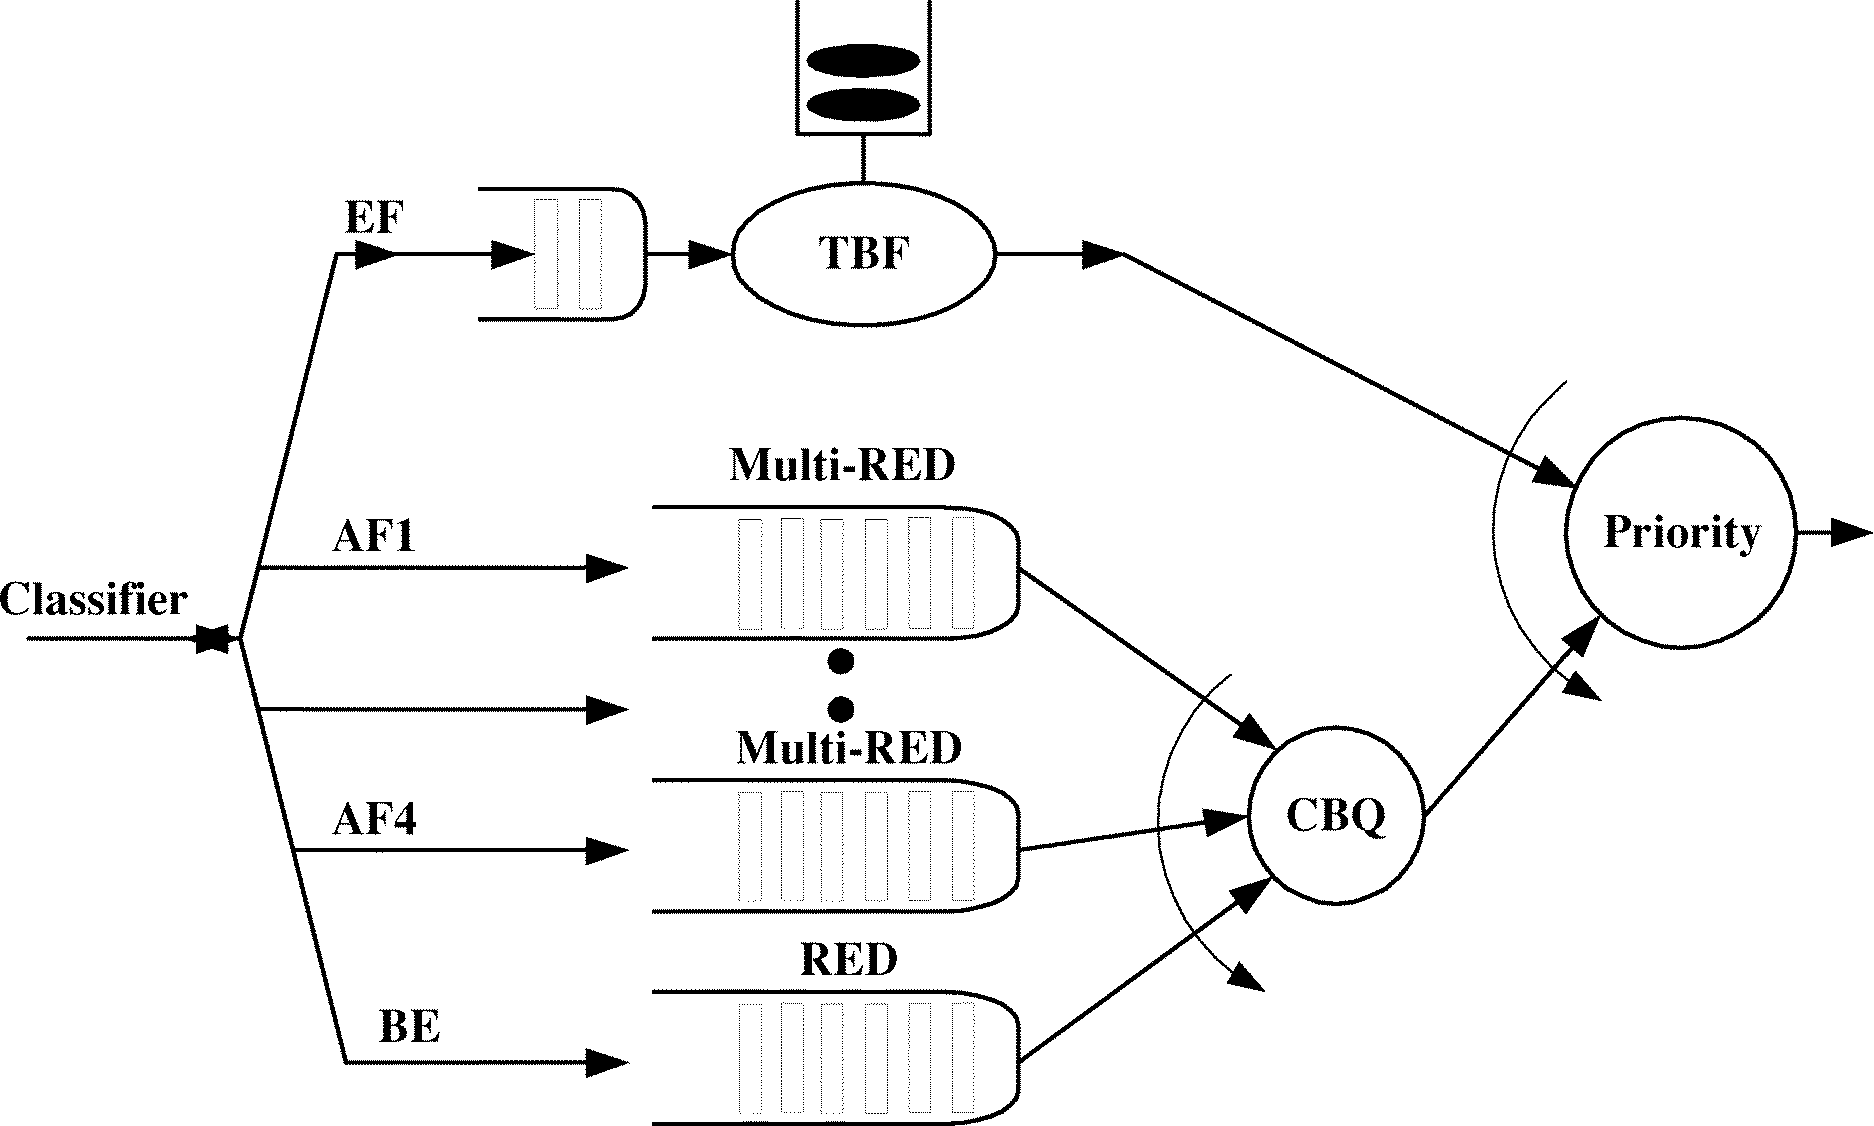
\includegraphics[width=8cm]{img/QoS_building-blocks.png}
	\caption{Implementation of QoS building blocks}
\end{figure}

\subsection{ATM}


\subsection{IP precedence and ToS}


\subsection{IntServ and RSVP}

\subsubsection{IntServ Model}
IntServ was designed to provide QoS to individual flows (or an individual session in case of multicast applications).

IntServ provisions virtual paths for each flow and sets up the required resources on these virtual paths. 

However, routing is not affected by these virtual paths, and they follow the default routing paths provided by the Internet routing protocols.
$\to$ It's done by using RSVP.


\paragraph{Warning} Routing is not affected by these virtual path because the reservation follows the entire route of the data packet.
\textbf{If route change, reservation is redone} (because of soft-state).


\subsubsection{Services classes}

IntServ services classes :
\begin{itemize}
	\item[-] Basic best-effort
	\item[+] Guaranteed Service (GS) : Used by applications that requires strict bounds on the e2e delay. It use a token bucket profile$(r,b)$ where 
	\begin{itemize}
		\item Minimum sending rate ($r$) 
		\item Minimum burst size of the traffic ($b$)
	\end{itemize}
	Routers allocate a forwarding rate of R for each session with a request if rate $< R$.
	\item[+] Controlled load (CL) : Experience small queueing delays, low loss and overall performance as if the network is not loaded.
\end{itemize}


\subsubsection{Reservation with RSVP}
\begin{enumerate}
	\item Sender sending \textbf{PATH message} (each 30sec) that carries :
	\begin{itemize}
		\item Tspec : Traffic specification object that describes the traffic profile. rate ($r$), bucket ($b$), peak rate ($p$), minimum unit ($m$) and max packet size ($M$).
		
		\item ADspec : Advertisement specification object which compute the accumulated QoS parameters along the e2e path.
		
		\item Phop : It's the path to join the receiver. The receiver just send by the reverse path.
		
		\begin{itemize}
			\item[Note:] There is a flowtable on each router to know the ``reverse'' path
		\end{itemize}
		
	\end{itemize}
	
	\item Receiver replies back with \textbf{RESV message} that carries :
	\begin{itemize}
		\item Rspec : Reservation specification
	\end{itemize}
	
	\item[Accepted] : if accepted by all routers along the path. $\to$ Setup actual reservation and filters on these router
	
	\item[Error] : corresponding router send PATHerr or RESVerr
	
	\item[End] : PATHtear and RESVtear message are sent to remove reservation states
\end{enumerate}


\paragraph{Filter}
\begin{itemize}
	\item Fixed filter :
	\item Shared filter :
	\item Wildcard filter :
\end{itemize}

\subsubsection{Evaluation of the IntServ model}


\subsection{Differentiated services}

\subsubsection{Background}


Packet are market on the edge router because their is lower bandwidth than on the ``center'' network. (= put the computation on the edge)

\subsubsection{IETF DiffServ Architecture}

\begin{itemize}
	\item Class selector : Using scheduling because class selector need a short delay point of view
	
	\begin{itemize}
		\item[Implementation]: Scheduling
	\end{itemize}
	
	\item Expedited forwarding : provide low delay, low loss, low jitter service.
	
	\textit{Backbone :} Priority queue with a token bucket on the higher priority queue to avoid starvation on the lower priority queue
	
	\textit{Edge :} Need also policing or shaping
	
	\begin{itemize}
		\item[Implementation]: WRR with $R_{EF}$ on EF queue and $R-R_{EF}$ on the other.
		
		Second solution is a WRR with $R-R_{EF}$ on EF queue and $R_{EF}$ on the other BUT with a Token Bucket on the EF queue. This solution have the same rate but their is a lower delay to forward packet.
	\end{itemize}
	
	\item Assured forwarding : 
	
	\begin{itemize}
		\item[Implementation]: With WRR
	\end{itemize}
	
\end{itemize}






\section{Multiprotocol Label Switching}


\begin{itemize}
	\item Label switching router :  that are capable of switching and routing packets on the basis of a label which has been appended to each packet
	
	\item Forwarding equivalence class :  Set of packet for which we have the same forwarding treatment
	
	\item Label switched path : unidirectional
	
\end{itemize}

MPLS header + field ?

\begin{itemize}
	\item Label value : 
	\item Exp : like DSCP
	\item S : To define the last element of the stack of label
	\item TTL : Time to live in hop
\end{itemize}

With the S bit, there is no limit to how many label attached to a packet.

MPLS is only IN the network, not on the host! (ingress node add MPLS, egress edge remove MPLS)

\subsection{Size label forwarding table}
Two possibly table :
\begin{enumerate}
	\item 20 inlabels, 3 inports, 4 outports, operation 
	
	We can make a differentiation with same label on different port.
	\item[OR]
	\item 20 inlabels, 3 outports, operation
	
	Lower information kept in memory.
\end{enumerate}



\subsection{Unique labels}

\begin{enumerate}
	\item Globally :
	\begin{itemize}
		\item 1 label = 1 path
		\item 1 label = 1 router
		\item 1 stack = 1 path
	\end{itemize}
	
	Drawback : all router need to know the label, minimum size of LFT
	Advantage : ?
	
	Actually, no use, but can change with ``SEGMENT ROUTING''
	
	\item Locally :
	\begin{itemize}
		\item 
	\end{itemize}
	
	Drawback : need to
	Label must be associated on router by DOWNSTREAM
	
	Advantage : different size for LTF, 
\end{enumerate}

\subsection{Forwarding equivalent classes}
\begin{enumerate}
	\item For example for voice traffic
	\item ?
\end{enumerate}

\section{Multicast with ipv6}
\subsection{IGMP (Internet Group Management Protocol)}
This is the protocol used between a router and end-users.  A end-user who wants to receive packets of a group can send a message to the router with IGMP. This protocol is never used between routers. 
\subsubsection{IGMPv1}
A user can send a request to join a group. The router will send a message every 60seconds to see if the user still wants packets from this group. Once it is done, if he wants to quit the group he has just to be silent to the messages of the router. After 3 non-response, the router will consider that the user has quit so the router won't forward anymore the packets of this group.
\subsubsection{IGMPv2}
A user can now send a leave message to the router. Once he receives a leave message the router send a request to the lan to see if someone still wants the packets of this group. If no-one responds, he won't forward the packets any more.
\subsubsection{IGMPv3}
A user can now request to receive only messages from some source(s) of a group.

\subsection{PIM}

\subsubsection{PIM DM}

\subsubsection{PIM SM}




\clearpage
\section{Abbreviations}
\begin{multicols}{2}
	\begin{description}
		\item[AF] Assured Forwarding
		\item[BA] Buffer Acceptance
		\item[BE] Best Effort
		\item[BGP] Border Gateway Protocol
		\item[CE] Client Edge router
		\item[DRR] Deficit Round-Robin
		\item[DSCP] Differentiated Services Code Point
		\item[DVMRP] Distance Vector Multicast Routing Protocol
		\item[ECMP] Equal Cost MultiPaths
		\item[EF] Expedited Forwarding
		\item[IGMP] Internet Group Management Protocol
		\item[ISP] Internet Service Provider
		\item[LDP] Label Distribution Protocol
		\item[LSP] Label Switching Path
		\item[MOSPF] Multicast Open Shortest Path First
		\item[MP-BGP] MultiProtocol Border Gateway Protocol
		\item[MPLS] MultiProtocol Label Switching
		\item[P] Provider router
		\item[PE] Provider Edge router
		\item[PIM] Protocol Independent Multicast
		\item[PIM DM] PIM Dense Mode
		\item[PIM SM] PIM Sparse Mode
		\item[RIP] Routing Information Protocol
		\item[RP] Rendez-vous Point
		\item[RPF] Reverse Path Forwarding
		\item[RSVP] Resource reSerVation Protocol
		\item[RSVP-TE] RSVP Traffic Engineering
		\item[RT] Route Target
		\item[SRLG] Shared Risk Link Groups
		\item[SSM] Source-Specific Multicast
		\item[VPN] Virtual Private Network
		\item[VRF] VPN Routing and Forwarding table
		\item[WDRR] Weighted Deficit Round-Robin
		\item[WFQ] Weighted Fair Queuing
	\end{description}
\end{multicols}

\end{document}
